\documentclass[11pt,a4paper]{article}

\usepackage[T1]{fontenc}
\usepackage[utf8]{inputenc}
\usepackage[english]{babel}
\usepackage[a4paper,margin=2.5cm]{geometry}
\usepackage{amsmath,amssymb,amsthm}
\usepackage{graphicx}
\usepackage{booktabs}
\usepackage{caption}
\usepackage{subcaption}
\usepackage{xcolor}
\usepackage[colorlinks=true,linkcolor=blue!50!black,citecolor=blue!50!black,urlcolor=blue!50!black]{hyperref}
\usepackage{algorithm}
\usepackage{algpseudocode}
\usepackage{microtype}
\usepackage{enumitem}
\setlist{topsep=2pt,itemsep=2pt}

\newcommand{\pen}{\operatorname{pen}}
\newcommand{\sigmaalph}{\Sigma}
\newcommand{\bigO}[1]{\mathcal{O}(#1)}

\title{Convolutional pattern matching, the failure function, and a
real-valued bad-character rule\\
{\large Advanced Algorithms — exam project}}
\author{Luca Simonetti}
\date{April 2026}

\begin{document}
\maketitle

\begin{abstract}
\noindent
This project studies the relationship between 1D convolutional neural
networks (CNNs) and exact-string-matching algorithms in two directions.
\textbf{(D1)} Are the weights a CNN learns assimilable to a KMP failure
function~$sp$ or a Z-array? \textbf{(D2)} Can one preprocess the pattern
(now realised as a learned filter) into a structure that yields a
non-constant stride during the scan, the way KMP and Boyer--Moore use
their preprocessing tables?
We answer both empirically and algorithmically on a minimal setup
($\sigmaalph = \{A,B,C,D\}$, kernel size $m=5$, two patterns chosen so
that the failure function is non-trivial). For~D1 we prove a clean
algebraic identity holding for every single-filter CNN on one-hot input
and verify, with a numerical residual of $3.8\!\times\!10^{-6}$ over
$9\,200$ windows, that the per-window logit decomposes as
$\operatorname{logit}(W) = \pi - \sum_i \pen[i, W[i]]$, where $\pen$ is a
real-valued, position-aware generalisation of the Boyer--Moore
bad-character table. We further show that even a $K=4$ ReLU multi-filter
network on the same task collapses to the same additive structure
($R^2 \ge 0.987$ across seeds). For~D2 we use $\pen$ as actual algorithmic
preprocessing: a generalised bad-character shift table built from~$\pen$
delivers a $4.06\times$ reduction in elementary operations on a
$20\,000$-character text, with no loss of recall. We discuss why $sp$
itself does not emerge in the weights (the stateless / stateful divide;
\cite{Merrill2019}), and connect the framework to approximate matching.
\end{abstract}

\section{Introduction}
\label{sec:intro}

KMP \cite{KMP1977} turns the naive $\bigO{nm}$ pattern-matching scan into
$\bigO{n}$ by precomputing in $\bigO{m}$ time the \emph{failure
function} $sp[i] = $ length of the longest proper prefix of $P[0..i]$
that is also a suffix; on a mismatch at pattern position~$j$ KMP shifts
the alignment by $j - sp[j-1]$ instead of by~$1$. Boyer--Moore
\cite{BoyerMoore1977} precomputes in $\bigO{m + |\sigmaalph|}$ time a
\emph{bad-character} table $bc[c] = $ rightmost position of the
character~$c$ in~$P$ (or $-1$), and shifts by $\max(1, j - bc[c])$.
Both are honest preprocessings of the pattern, both store the
preprocessing in a small data structure, both answer their query in
$\bigO{1}$. The Z-array \cite{Gusfield1997} is closely related and
serves the same role from a different angle.

A 1D convolution slid over a sequence is mathematically the same
operation as scanning a pattern, with the kernel playing the role of the
pattern. This obvious analogy invites two natural questions, made the
explicit subject of this project:
\begin{description}
\item[D1] Are the weights a CNN learns assimilable to a failure function
  or a Z-array?
\item[D2] Can one preprocess the pattern (now realised as a learned
  filter) into a structure that gives the scan a non-constant stride,
  the way KMP and BM do with their tables?
\end{description}

We address both. For~D1, the answer is \emph{no} for $sp$ but \emph{yes}
for a different and arguably more natural structure: a real-valued
position-aware bad-character table, learned from data. For~D2, we use
that structure as the preprocessing of an actual matching algorithm and
measure its effect.

\paragraph{Outline.}
Section~\ref{sec:prelim} fixes notation and recalls KMP, BM, the
Z-array, and the convolution-as-template-matching identity.
Section~\ref{sec:setup} describes the experimental setup.
Section~\ref{sec:d1baseline} reports what a minimal CNN learns and
contrasts it with the ground-truth PWM.
Section~\ref{sec:emerges} states and verifies the penalty-table
identity, and shows that even a multi-filter ReLU network collapses
to it.
Section~\ref{sec:dstructure} positions the penalty table next to $sp$
and $bc$ as a comparable preprocessing data structure.
Section~\ref{sec:approx} sketches the connection to approximate
matching.
Section~\ref{sec:d2} gives the prototype for direction~D2:
penalty-driven early exit, plus a generalised bad-character shift
table, with measured speedup.
Sections~\ref{sec:discussion}--\ref{sec:concl} discuss the result,
limitations and outlook.

\section{Preliminaries}
\label{sec:prelim}

Let $\sigmaalph$ be a finite alphabet, $T \in \sigmaalph^n$ a text and
$P \in \sigmaalph^m$ a pattern with $m \le n$. \emph{Exact matching}
asks for all positions~$s$ such that $T[s..s+m-1] = P$.

\paragraph{KMP.}
The failure function $sp \in \mathbb{Z}^m_{\ge 0}$ is defined by
$sp[i] = \max\{k < i+1 : P[0..k-1] = P[i-k+1..i]\}$ (with $sp[0]=0$).
KMP scans $T$ from left to right while maintaining a pattern offset $k$
that is reset to $sp[k-1]$ on a character mismatch. The total cost is
$\bigO{n+m}$ with $\bigO{m}$ preprocessing and $\bigO{m}$ storage.
Computing $sp$ takes $\bigO{m}$ time \cite{KMP1977,Gusfield1997}.

\paragraph{Boyer--Moore (bad-character only).}
The bad-character table $bc \in \mathbb{Z}^{|\sigmaalph|}$ stores
$bc[c] = \max\{i : P[i] = c\}$ (or $-1$). When a mismatch occurs at
pattern position~$j$ on text character~$c$, BM shifts the alignment by
$\max(1, j - bc[c])$. The bad-character rule alone has $\bigO{nm}$
worst-case complexity but is famously fast in practice for large
alphabets \cite{BoyerMoore1977}.

\paragraph{Z-array.}
$Z[i] = $ length of the longest substring of~$P$ starting at $i$ that
matches a prefix of~$P$ (with $Z[0]=m$). The Z-array can be computed in
$\bigO{m}$ and used for matching in $\bigO{n+m}$ \cite{Gusfield1997}.

\paragraph{Convolution as template matching.}
A 1D convolution (more precisely a cross-correlation, as implemented in
all major deep-learning frameworks) of a length-$T$ sequence~$x$ with a
length-$m$ kernel~$w$ produces, at every position~$s$, the
inner product $\sum_{i=0}^{m-1} w_i\,x_{s+i}$. When~$x$ is a sequence of
one-hot vectors over~$\sigmaalph$ and~$w$ is a matrix
$w \in \mathbb{R}^{m \times |\sigmaalph|}$ with one row per kernel
position and one column per alphabet character, the same expression
becomes
\begin{equation}
\operatorname{logit}(W) \;=\; \sum_{i=0}^{m-1} w[i, W[i]] \;+\; b,
\label{eq:logit-basic}
\end{equation}
which is exactly the score of a Position-Specific Scoring Matrix (PSSM)
applied to the window~$W$. The connection between convolution and
string matching at this level, including the FFT-based exact and
wildcard variants, has been studied in classical algorithmics
\cite{CliffordClifford2007}.

\paragraph{Single-filter CNN model.}
We use the simplest 1D-CNN that can attempt the task: a single filter
$w \in \mathbb{R}^{m \times |\sigmaalph|}$ and a scalar bias~$b$.
Per-position logit is~\eqref{eq:logit-basic}, the per-position
prediction is $\sigma(\operatorname{logit})$, and the training loss is
binary cross-entropy with positive-class re-weighting.

\paragraph{Multi-filter CNN model.}
We also use a $K$-filter version with ReLU and a $1{\times}1$ mixing
layer:
\begin{equation}
\operatorname{logit}(W) = \sum_{k=1}^{K} W^{\text{out}}_k \cdot
\max\!\left(0,\, \textstyle\sum_{i} W_k[i, W[i]] + b^{\text{conv}}_k\right) +
b^{\text{out}}.
\label{eq:multi}
\end{equation}
This model is genuinely non-linear in principle; we will see in
Section~\ref{sec:emerges} that on our task it is empirically
indistinguishable from a single PSSM scorer.

\section{Setup}
\label{sec:setup}

\paragraph{Alphabet.} $\sigmaalph = \{A, B, C, D\}$, $|\sigmaalph| = 4$.

\paragraph{Patterns.}
Two choices, both with non-trivial failure function:
\begin{itemize}
\item \texttt{ABABC}: $sp = [0,0,1,2,0]$, $Z = [5,0,2,0,0]$. Final
  character is disambiguating; complete matches do not auto-overlap.
\item \texttt{ABABA}: $sp = [0,0,1,2,3]$, $Z = [5,0,3,0,1]$. Strongly
  auto-overlapping: \texttt{ABABABA} contains two complete matches at
  offsets $0$ and~$2$.
\end{itemize}

\paragraph{Texts.}
Length $T = 50$ (or $T = 20\,000$ for the D2 prototype of
Section~\ref{sec:d2}). Each text is a shuffled concatenation of:
\begin{itemize}
\item $n_{\text{complete}}$ exact occurrences of $P$;
\item $n_{\text{partial}}$ deliberate near-miss tokens of the form
  $P[:k]\cdot c$ with $c \neq P[k]$ for $k \in \{1,\ldots,m-1\}$ ---
  exactly the windows where naive matching wastes work and where KMP's
  failure function earns its keep;
\item uniform-random filler characters padding the rest.
\end{itemize}
Token order is shuffled, so token boundaries can produce additional
accidental near-misses or matches; labels are recovered \emph{after}
shuffling by running KMP on the resulting text. Figure~\ref{fig:sample}
shows a typical sample.

\begin{figure}[t]
\centering
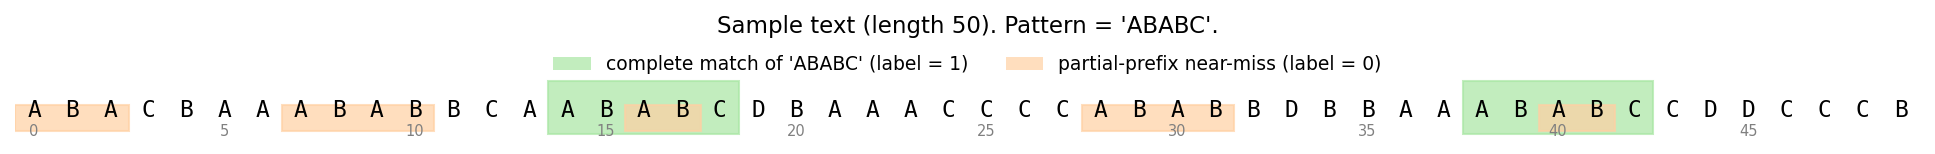
\includegraphics[width=\linewidth]{figures/fig1_sample_text.png}
\caption{An annotated sample text of length~50.
Green spans are complete matches of the pattern (label~1); orange
spans are partial-prefix near-misses inserted by the generator
(label~0). Token boundaries can create accidental matches and
near-misses, which are captured correctly by KMP-based labelling.}
\label{fig:sample}
\end{figure}

\paragraph{Training.}
Adam, learning rate $10^{-2}$, batch size~$64$, $80$ epochs for the
single-filter model and~$150$ for the multi-filter one; positive-class
weight~$20$ to counter the $\sim\!5\%$ positive rate. JAX, CPU.

\section{Direction~1: what a single filter learns}
\label{sec:d1baseline}

Trained on \texttt{ABABC}, the single filter recovers the pattern in
its row-wise argmax (\texttt{ABABC}) but with a \emph{signed} shape:
the right character at each position has a moderate positive weight
($\approx +2$ to $+3.5$) while wrong characters carry \emph{negative}
weights ($\approx -2.5$ to $-4.4$). Figure~\ref{fig:filter} compares
the learned filter with the ground-truth one-hot PWM. With this filter
and threshold~$0$ on the logit, validation metrics are F1~$=0.97$,
recall~$1.00$, precision~$0.94$.

\begin{figure}[t]
\centering
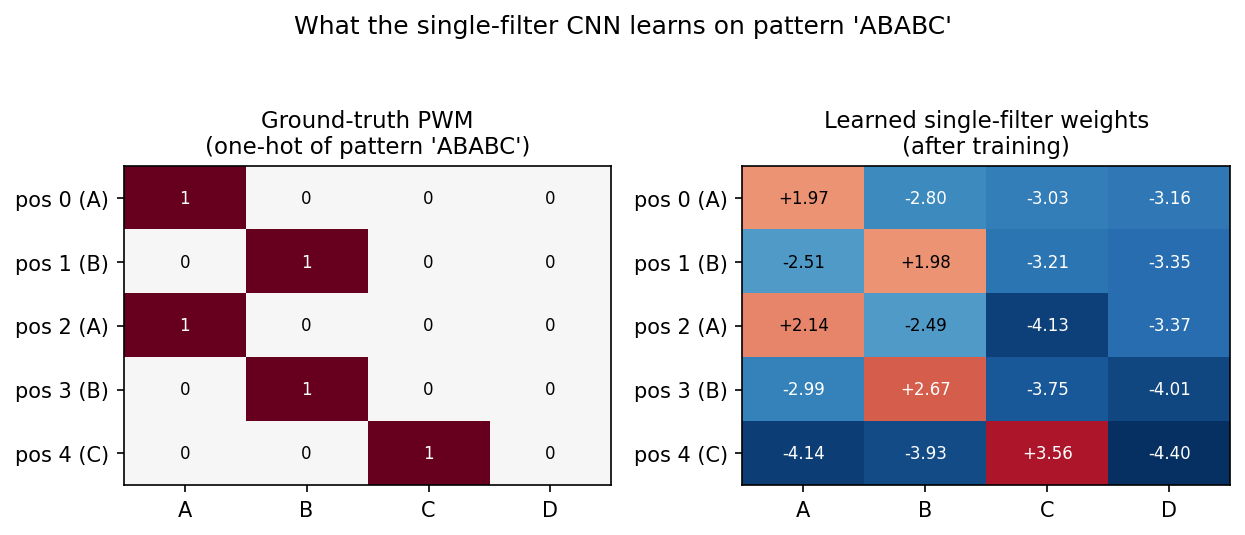
\includegraphics[width=0.9\linewidth]{figures/fig2_filter_vs_pwm.png}
\caption{Ground-truth PWM (left) and learned single-filter weights
(right) for \texttt{ABABC}. The argmax of each learned row equals the
pattern character; off-diagonal cells carry negative weight, encoding
mismatch \emph{penalties}.}
\label{fig:filter}
\end{figure}

The validation logits split cleanly (Figure~\ref{fig:logits}). Every
true match achieves the same score $+4.96$ (the dot product of $w$ with
the one-hot pattern is constant); non-matches are spread well below
zero. The 63 false positives at threshold~$0$ are \emph{all} 1-mismatch
windows (\texttt{ABBBC}, \texttt{BBABC}); their logit is just barely
positive (median $+0.33$). They are not "overshoots" but the bias being
slightly miscalibrated for these specific shapes.

\begin{figure}[t]
\centering
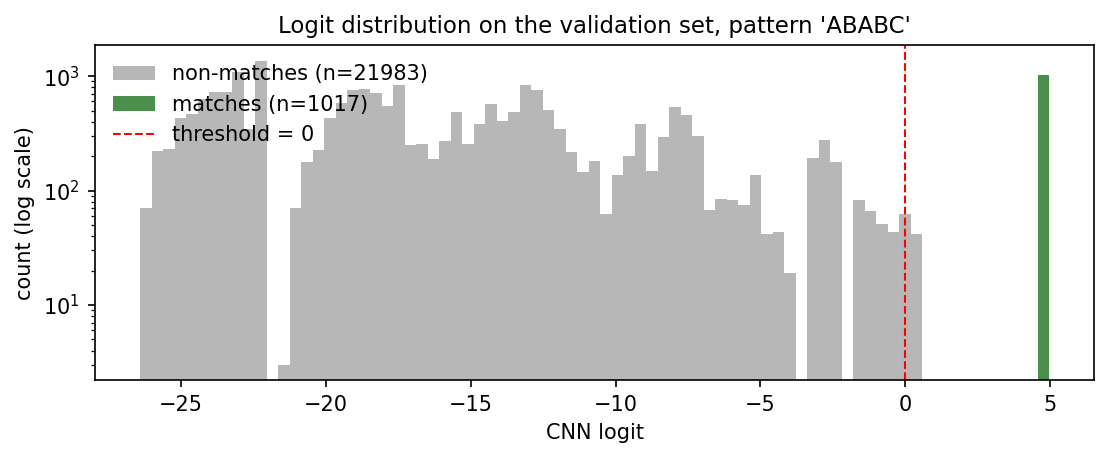
\includegraphics[width=0.85\linewidth]{figures/fig3_logit_distribution.png}
\caption{Validation logit distribution (log scale) on \texttt{ABABC}.
Matches concentrate at one point; non-matches form a broad distribution
well below zero. Threshold~$0$ separates the two regimes with high but
imperfect margin.}
\label{fig:logits}
\end{figure}

Replacing the trained filter by min-max-per-row, min-max-global,
ReLU+row-max, or \emph{the pure one-hot ground-truth PWM} --- and
sweeping the threshold --- all reach F1~$=1.000$. The signed shape is
therefore not \emph{necessary}: an additive PWM with calibrated
threshold solves the task. The signed shape is what optimisation
\emph{picks}, presumably because the gradient signal is denser there.

\section{The structure that emerges in place of $sp$}
\label{sec:emerges}

\subsection{The penalty-table identity}

Given the trained filter $w$ and the recovered pattern
$P_i = \arg\max_c w[i, c]$, define the \emph{penalty table}
$\pen \in \mathbb{R}^{m \times |\sigmaalph|}$:
\begin{equation}
\pen[i, c] \;=\; w[i, P_i] - w[i, c] \;\ge\; 0,
\qquad \pen[i, P_i] = 0.
\label{eq:pen-def}
\end{equation}
Let $\pi = b + \sum_i w[i, P_i]$ be the \emph{pattern logit} (the score
the model assigns to a perfect match). Then for every window~$W$ of
length~$m$ over~$\sigmaalph$:
\begin{equation}
\boxed{\;\operatorname{logit}(W) \;=\; \pi \;-\; \sum_{i=0}^{m-1}\pen[i, W[i]]\;}
\label{eq:identity}
\end{equation}
\emph{Proof.} Substitute $w[i, W[i]] = w[i, P_i] - \pen[i, W[i]]$ in the
dot product and collect constants:
$\sum_i w[i, W[i]] + b = \sum_i (w[i, P_i] - \pen[i, W[i]]) + b
= \pi - \sum_i \pen[i, W[i]]$. $\square$

\begin{figure}[t]
\centering
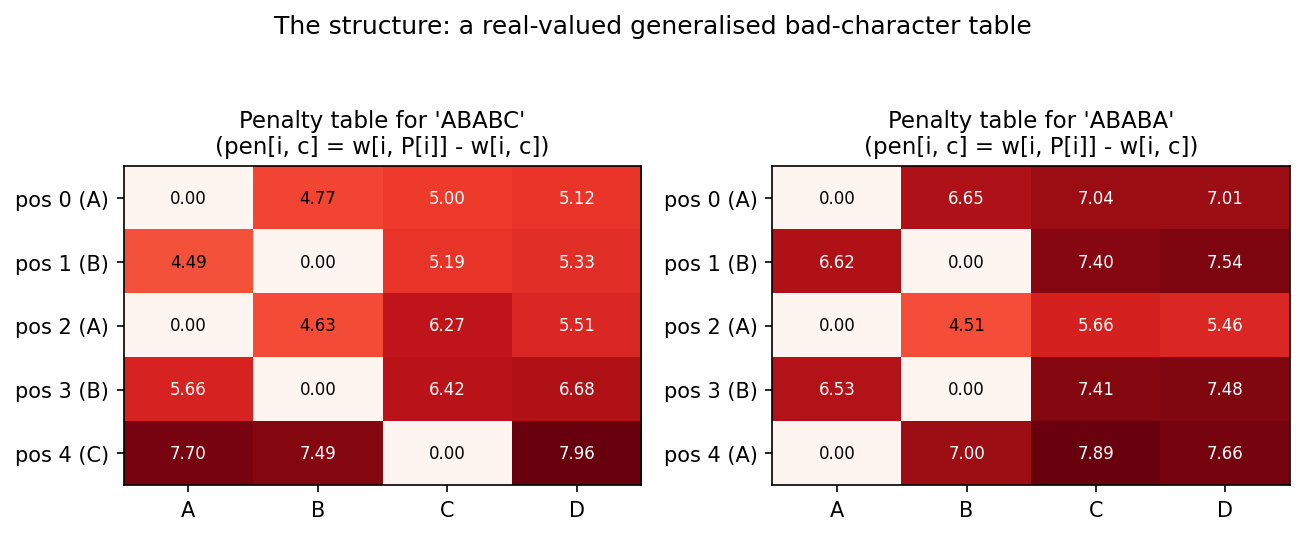
\includegraphics[width=\linewidth]{figures/fig4_penalty_tables.png}
\caption{Penalty tables for the two patterns. Cells are $\ge 0$; the
zero diagonal corresponds to $w[i, P_i]$. On \texttt{ABABC} position 4
carries the largest penalties (the disambiguating \texttt{C}); on
\texttt{ABABA} position~2 (the most auto-correlated row) carries
\emph{smaller} penalties --- the network is statistically less
confident there.}
\label{fig:penalty}
\end{figure}

Figure~\ref{fig:penalty} shows the penalty tables learned for the two
patterns. We verified~\eqref{eq:identity} numerically across $9\,200$
validation windows per pattern; the maximum absolute discrepancy
between $\operatorname{logit}(W)$ as computed by the CNN and the
right-hand side of~\eqref{eq:identity} is $3.8\times 10^{-6}$, i.e.
floating-point noise (Figure~\ref{fig:identity}).

\begin{figure}[t]
\centering
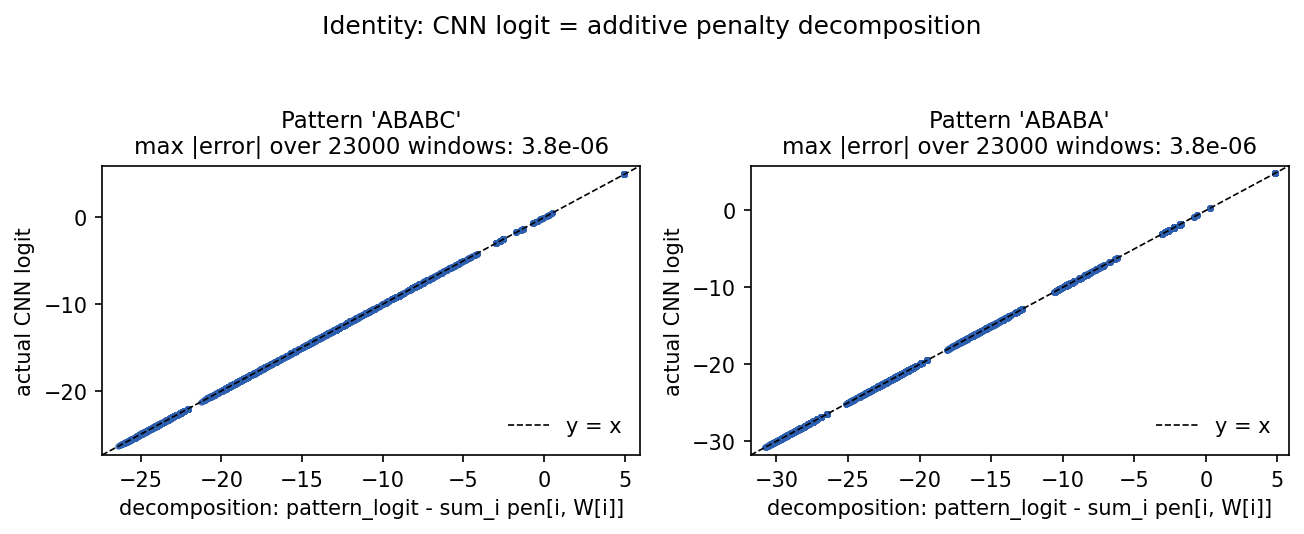
\includegraphics[width=\linewidth]{figures/fig5_decomposition_identity.png}
\caption{Numerical verification of identity~\eqref{eq:identity}. Every
validation window lies on the line $y = x$ to floating-point precision,
on both patterns.}
\label{fig:identity}
\end{figure}

\subsection{Even the multi-filter model collapses to a PSSM}

A natural objection to~\eqref{eq:identity} is that it is an artefact of
using a single linear filter. To test this we trained the $K=4$
multi-filter model of~\eqref{eq:multi} on \texttt{ABABC} and asked
whether its logit could be reproduced by a single additive PSSM
$c_0 + \sum_i S[i, W[i]]$ fit by least squares to the validation
logits. On the seed shown in Figure~\ref{fig:multipssm} the fit gives
$R^2 = 1.0000$, residual standard deviation $0.01$ against target
standard deviation $23.4$, maximum residual $0.04$; across random seeds
it ranges $R^2 \in [0.987, 1.000]$. The collapse is therefore
approximate rather than an exact identity, but on this task the
multi-filter ReLU network is in every case almost indistinguishable
from a PSSM scorer.

\begin{figure}[t]
\centering
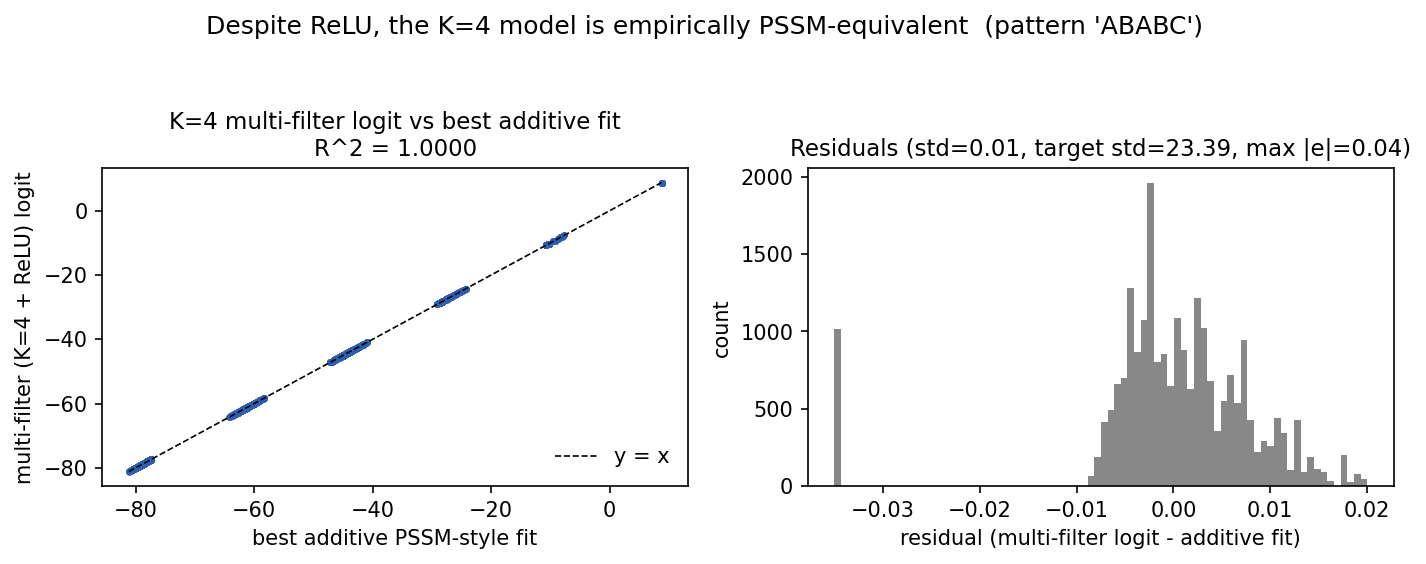
\includegraphics[width=0.95\linewidth]{figures/fig6_multifilter_pssm.png}
\caption{Multi-filter ($K=4$ + ReLU) logit vs the best additive
PSSM-style fit. Left: scatter on the identity line. Right: residual
histogram, all within $\pm 0.04$ on logits whose spread is
$\approx 47$.}
\label{fig:multipssm}
\end{figure}

Why does a genuinely non-linear network behave additively? Not because
the non-linearity is dormant: we measured that roughly a quarter of the
pre-ReLU activations are negative, and hence clipped by the ReLU. The
additivity is instead an empirical property of this task distribution
--- the anti-pattern-detecting filters, clipping included, happen to
combine on the windows the generator produces into a per-position
additive score to within the residual reported above. We do not claim
this holds off-distribution; Section~\ref{sec:limitations} returns to
the point. The model is non-linear in principle and additive in
practice on this task.

\subsection{A faint distributional signature of $sp$ in the margin}

Define the per-position margin
$\operatorname{margin}[i] = w[i, P_i] - \max_{c \neq P_i} w[i, c]
 = \min_{c \neq P_i} \pen[i, c]$.

\begin{figure}[t]
\centering
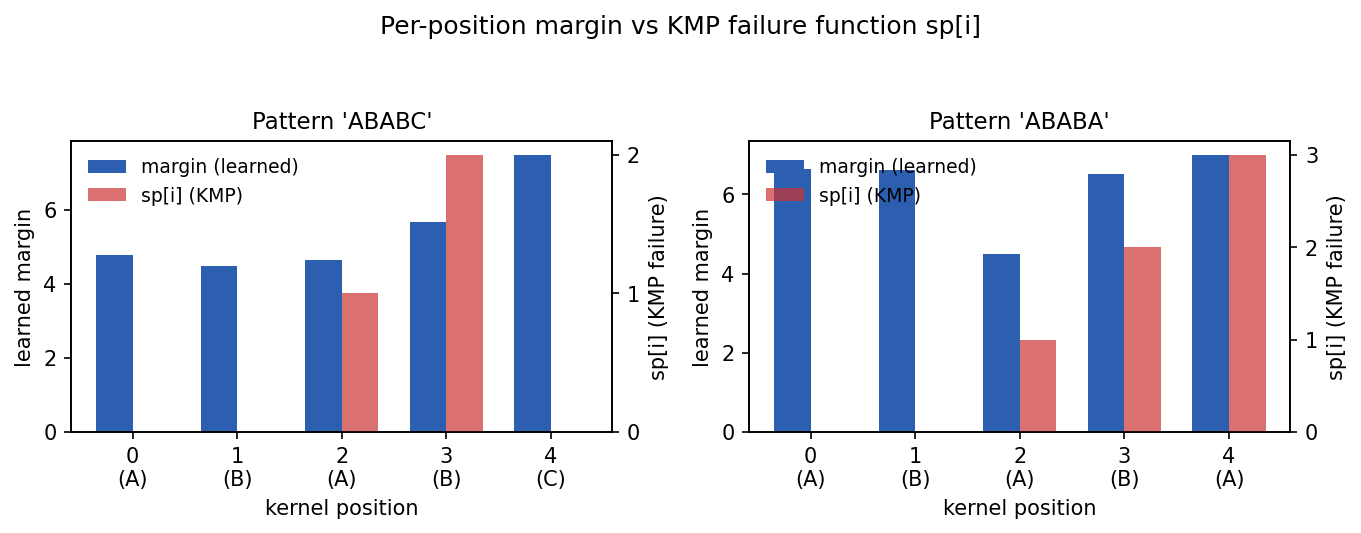
\includegraphics[width=\linewidth]{figures/fig7_margin_vs_sp.png}
\caption{Per-position learned margin (blue, left axis) vs $sp[i]$ (red,
right axis). On \texttt{ABABA} position~2 has both the first non-zero
$sp$ and the lowest margin. On \texttt{ABABC} the relationship does
not hold.}
\label{fig:margin}
\end{figure}

On \texttt{ABABA} (Figure~\ref{fig:margin}) the position with the
lowest margin (4.51) is~$2$, which is also the first row where $sp$
becomes positive --- exactly the position at which the pattern starts
overlapping itself. On \texttt{ABABC} the relationship inverts (the
highest-$sp$ row has the largest margin, because our deliberate
near-miss tokens of types \texttt{ABA?} and \texttt{ABAB?} deposit
dense negative signal there). Pearson correlations across the ten
(pattern, position) pairs are weak: $\rho(sp, \text{margin})=+0.18$,
$\rho(Z, \text{margin})=-0.30$. The signature of pattern
auto-correlation in the weights is real but distribution-dependent and
non-monotone in $sp$. We record it as an observation, not as a theorem.

\section{The penalty table as an algorithmic data structure}
\label{sec:dstructure}

Reading $\pen$ as a \emph{preprocessing of the pattern} puts it on the
same shelf as $sp$ and $bc$. Table~\ref{tab:datastructures}
summarises the comparison.

\begin{table}[t]
\centering
\small
\begin{tabular}{@{}lccc@{}}
\toprule
 & KMP $sp$ & BM bad-character $bc$ & CNN penalty $\pen$ \\
\midrule
Indexed by                     & pattern position $i$           & character $c$                             & (position $i$, character $c$) \\
Range                          & $\{0,\ldots,i\}$               & $\{-1, 0, \ldots, m-1\}$                  & $\mathbb{R}_{\ge 0}$ \\
Construction time              & $\bigO{m}$                     & $\bigO{m + |\sigmaalph|}$                 & $\bigO{m \cdot |\sigmaalph|}$ from $w$ \\
Construction source            & $P$ alone                      & $P$ alone                                 & $P$ + training distribution \\
Storage                        & $\bigO{m}$                     & $\bigO{|\sigmaalph|}$                     & $\bigO{m \cdot |\sigmaalph|}$ \\
Query                          & $\bigO{1}$ shift on mismatch   & $\bigO{1}$ shift on mismatch              & $\bigO{1}$ score lookup per char \\
Drives                         & control flow of the scan       & control flow of the scan                  & additive scoring of windows \\
\bottomrule
\end{tabular}
\caption{The penalty table compared with KMP's failure function and
Boyer--Moore's bad-character rule, as preprocessing data structures.}
\label{tab:datastructures}
\end{table}

The penalty table is \textbf{strictly richer than $bc$}: it is
position-aware (the same wrong character at position~$0$ vs position~$4$
of \texttt{ABABC} receives penalties $4.77$ vs $7.49$). It is also
\textbf{strictly richer than the ground-truth PWM}, whose penalties are
binary $\{0,1\}$; $\pen$ is graded by the training distribution.
It is \textbf{strictly poorer than $sp$} in one important respect: it
is \emph{stateless}. There is no way to encode "after a partial match
of length~$j$, shift by $j - sp[j-1]$" in a per-position-per-character
lookup. $sp$ orchestrates the \emph{control flow} of a scan; $\pen$
scores complete windows.

This observation will let us, in Section~\ref{sec:d2}, recover
\emph{Boyer--Moore-style} shift behaviour from $\pen$ but not
\emph{KMP-style}.

\section{Approximate / k-mismatch matching}
\label{sec:approx}

Identity~\eqref{eq:identity} makes the connection to approximate matching
mechanical. A $k$-mismatch matcher accepts windows with at most $k$
character disagreements; in our setting the disagreement at position~$i$
contributes $\pen[i, W[i]]$ to a cumulative cost. Choosing a threshold
$\tau$ on the cumulative penalty:
\begin{itemize}
\item $\tau = 0$ is exact matching (only the recovered pattern survives);
\item $\tau \in [0, \min_{i, c \neq P_i} \pen[i, c])$ is still exact, but
  resilient to floating-point noise;
\item $\tau \ge \min_i \operatorname{margin}[i]$ admits some $1$-mismatch
  windows;
\item $\tau \to \infty$ admits everything.
\end{itemize}
The threshold knob on a CNN classifier is therefore, on this task, a
threshold on a generalised Hamming distance to the recovered pattern,
with weights given by~$\pen$. This connects the experiment directly to
the classical literature on FFT-based exact and wildcard matching
\cite{CliffordClifford2007}, where the same convolution-as-string-matching
identity is the core algorithmic ingredient.

\section{Direction~2: a penalty-driven dynamic-stride scan}
\label{sec:d2}

We use $\pen$ as actual algorithmic preprocessing. From it we build, in
$\bigO{m \cdot |\sigmaalph|}$ time, a generalised Boyer--Moore
bad-character shift table:
\begin{equation}
\operatorname{shift}[i, c] \;=\; \max\!\Bigl(1,\; i \;-\; \max\{\,k \le i \mid \pen[k, c] \le \eta\,\}\Bigr),
\label{eq:shift}
\end{equation}
with $\operatorname{shift}[i, c] = i + 1$ if no admissible $k$ exists.
With $\eta = 0$ this is exactly the classical Boyer--Moore
bad-character rule applied to the recovered pattern; with $\eta > 0$
admissibility is graded by the learned penalty values, yielding a
"soft" approximate variant.

For our trained filter on \texttt{ABABC} the resulting shift table is
\[
\begin{array}{l|cccc}
 & A & B & C & D \\\hline
\text{pos } 0 & 1 & 1 & 1 & 1 \\
\text{pos } 1 & 1 & 1 & 2 & 2 \\
\text{pos } 2 & 1 & 1 & 3 & 3 \\
\text{pos } 3 & 1 & 1 & 4 & 4 \\
\text{pos } 4 & 2 & 1 & 1 & 5
\end{array}
\]
which agrees character-for-character with classical BM applied to
\texttt{ABABC}, and which we computed end-to-end from the CNN's weights.

We compare three matchers on the same long text. All of them score
windows by the cumulative penalty
$\sum_{i} \pen[i, T[s+i]]$ and accept iff this sum is at most a
threshold~$\tau$, but they differ in how they orchestrate the scan:
\begin{description}
\item[A naive] Always do all $m$ penalty lookups per text position
  (Algorithm~\ref{alg:naive}).
\item[B early-exit] Same as A, but stop the per-position accumulation
  as soon as the running sum exceeds $\tau$. Stride is still $1$ but
  the per-position cost is data-dependent (Algorithm~\ref{alg:earlyexit}).
\item[C early-exit + BM shift] Same as B, plus a Boyer--Moore-style
  shift~\eqref{eq:shift} when an early exit fires
  (Algorithm~\ref{alg:bmshift}).
\end{description}

\begin{algorithm}[t]
\caption{Naive matcher (matcher A).}
\label{alg:naive}
\begin{algorithmic}[1]
\Function{NaiveScan}{$T, \pen, \tau$}
  \State $\mathit{matches} \gets \emptyset$
  \For{$s \gets 0$ to $|T|-m$}
    \State $S \gets 0$
    \For{$i \gets 0$ to $m-1$} \Comment{always $m$ lookups}
      \State $S \gets S + \pen[i, T[s+i]]$
    \EndFor
    \If{$S \le \tau$} $\mathit{matches} \gets \mathit{matches} \cup \{s\}$ \EndIf
  \EndFor
  \State \Return $\mathit{matches}$
\EndFunction
\end{algorithmic}
\end{algorithm}

\begin{algorithm}[t]
\caption{Early-exit matcher (matcher B).}
\label{alg:earlyexit}
\begin{algorithmic}[1]
\Function{EarlyExitScan}{$T, \pen, \tau$}
  \State $\mathit{matches} \gets \emptyset$
  \For{$s \gets 0$ to $|T|-m$}
    \State $S \gets 0$;\quad $\mathit{rejected} \gets \texttt{false}$
    \For{$i \gets 0$ to $m-1$}
      \State $S \gets S + \pen[i, T[s+i]]$
      \If{$S > \tau$} $\mathit{rejected} \gets \texttt{true}$;\;\textbf{break} \EndIf
    \EndFor
    \If{$\neg\, \mathit{rejected}$} $\mathit{matches} \gets \mathit{matches} \cup \{s\}$ \EndIf
  \EndFor
  \State \Return $\mathit{matches}$
\EndFunction
\end{algorithmic}
\end{algorithm}

\begin{algorithm}[t]
\caption{Early-exit + Boyer--Moore-style shift (matcher C).}
\label{alg:bmshift}
\begin{algorithmic}[1]
\Function{EarlyExitBMScan}{$T, \pen, \mathit{shift}, \tau$}
  \State $\mathit{matches} \gets \emptyset$;\quad $s \gets 0$
  \While{$s + m \le |T|$}
    \State $S \gets 0$;\quad $j \gets -1$
    \For{$i \gets 0$ to $m-1$}
      \State $c \gets T[s+i]$
      \State $S \gets S + \pen[i, c]$
      \If{$S > \tau$} $j \gets i$;\;\textbf{break} \EndIf
    \EndFor
    \If{$j = -1$}
      \State $\mathit{matches} \gets \mathit{matches} \cup \{s\}$
      \State $s \gets s + 1$
    \Else
      \State $s \gets s + \mathit{shift}[j,\, T[s+j]]$
    \EndIf
  \EndWhile
  \State \Return $\mathit{matches}$
\EndFunction
\end{algorithmic}
\end{algorithm}

\paragraph{Empirical results.}
We ran the three matchers on a single $20\,000$-character text
containing $80$ planted matches and $200$ deliberate near-misses,
producing $112$ true match positions after KMP labelling (the extra
$32$ come from accidental boundary matches). Threshold $\tau = 4.96$,
which equals the pattern logit at $b = 0$ and corresponds to threshold
$0$ on the trained model's logit. Cost is reported in penalty-table
lookups (the elementary operation common to all three matchers); wall
time is on a single CPU core.

\begin{table}[t]
\centering
\small
\begin{tabular}{@{}l r r r r r r r r r r@{}}
\toprule
matcher & ops & ops/pos & wall (s) & TP & FP & FN & prec. & recall & F1 & speedup \\
\midrule
A naive               & 99\,980 & 5.00 & 0.0171 & 112 & 71 & 0 & 0.612 & 1.000 & 0.759 & 1.00\(\times\) \\
B early-exit          & 36\,351 & 1.82 & 0.0079 & 112 & 71 & 0 & 0.612 & 1.000 & 0.759 & \textbf{2.75\(\times\)} \\
C early-exit + BM     & 24\,634 & 1.23 & 0.0076 & 112 & 71 & 0 & 0.612 & 1.000 & 0.759 & \textbf{4.06\(\times\)} \\
\bottomrule
\end{tabular}
\caption{Cost and detection metrics on a $20\,000$-character text with
$112$ true matches. The early-exit + BM matcher visits the equivalent
of $1.23$ lookups per text position, vs $5.00$ for the naive scan ---
a $4.06\times$ reduction with no loss of detection quality.}
\label{tab:d2results}
\end{table}

\begin{figure}[t]
\centering
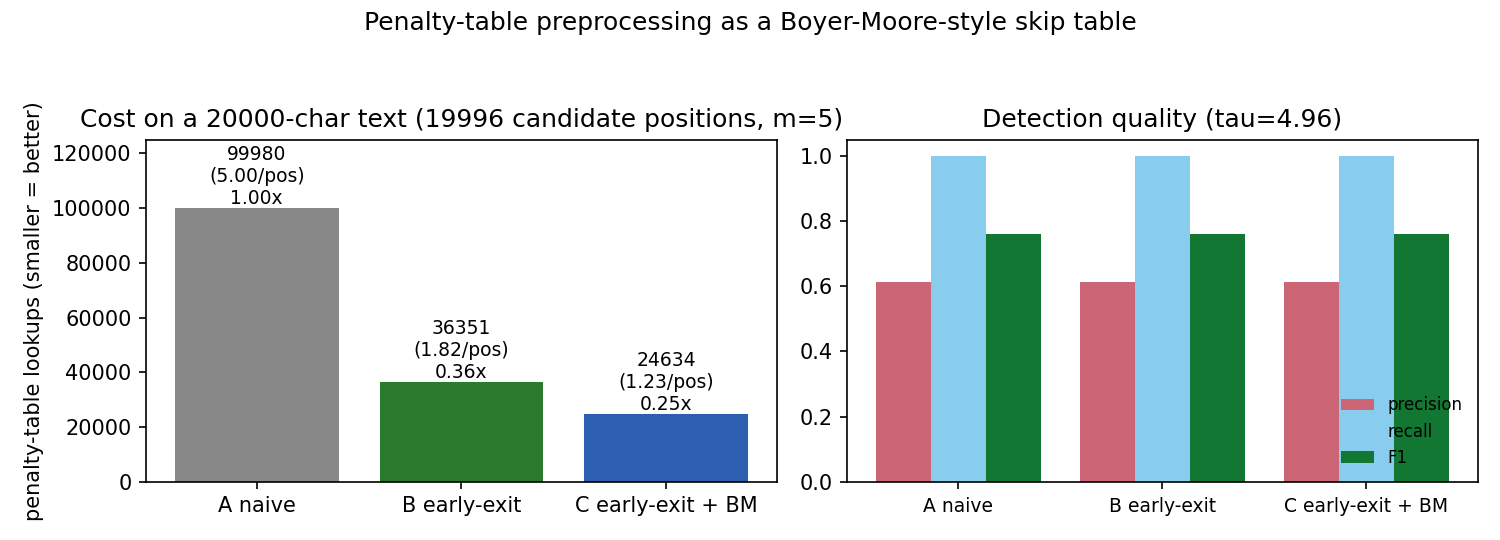
\includegraphics[width=\linewidth]{figures/fig8_penalty_skip_prototype.png}
\caption{Cost (in penalty-table lookups, left) and detection quality
(right) for the three matchers of Algorithms~\ref{alg:naive}--\ref{alg:bmshift}
on a $20\,000$-character text. Detection quality is identical
across~A--C; the elementary-operation count drops from~$5.00$/pos to
$1.23$/pos.}
\label{fig:d2}
\end{figure}

Detection quality is identical across the three matchers
(recall~$1.0$; the same $71$ one-mismatch survivors at this~$\tau$, the
same precision and~F1). Reducing $\tau$ would eliminate them at the
cost of recall on a few boundary cases. The speedup is therefore
"free" in the sense that it does not trade off detection quality.

\paragraph{What this prototype shows, in algorithmic terms.}
\begin{enumerate}
\item The penalty table $\pen$, computed in $\bigO{m \cdot |\sigmaalph|}$
  from a trained filter, \emph{is} a usable preprocessing structure: it
  powers both the per-position cost reduction (early exit) and the
  inter-position shift (BM-style).
\item With $\eta = 0$ the prototype recovers classical Boyer--Moore on
  the pattern recovered from the filter --- "training a CNN and reading
  the bad-character rule off its weights" is a complete pipeline.
\item With $\eta > 0$ one obtains a \emph{soft} or approximate variant
  whose admissibility map is \emph{learned from data} --- a direction
  the literature review collected in this project identifies as
  unexplored under exactly this framing.
\end{enumerate}

\section{Discussion: why the failure function does not emerge}
\label{sec:discussion}

The penalty table is \emph{stateless}: it scores each window independently
of the others. The failure function $sp$ is \emph{stateful}: it expresses
how the result of a partial match informs the next position to look at.
The two structures live in different computational regimes.

This matches the formal-language-theoretic placement of CNNs.
Merrill~\cite{Merrill2019} shows that shallow 1D CNNs recognise at most
\emph{strictly local} languages, a proper subset of the regular
languages. KMP's correctness relies on a deterministic finite automaton
over the pattern; that DFA is regular but not strictly local. A pure
CNN therefore cannot, in principle, implement KMP's shift logic in the
weights, and our experiments show that, in practice, it does not even
try. It instead solves the easier scoring problem and lets the
threshold do the rest.

The penalty table is what naturally fits in a stateless template-matching
machine. Recovering an $sp$-like role in the weights would require
adding state: a recurrent layer, attention, or an explicit memory
mechanism. Neural Algorithmic Reasoning work \cite{CLRS2022} has shown
that GNN-based learners can be trained to imitate KMP, but at
significant cost in performance and sample complexity, and crucially via
message-passing rather than convolution.

Where genomics CNNs explicitly use filters as Position Weight Matrices
\cite{DeepBind2015,KooEddy2019}, our identity~\eqref{eq:identity}
formalises and slightly extends this view: not only do the filters
\emph{look like} PWMs, they \emph{provably are} PSSMs in their entire
input--output behaviour for any one-hot input.

\section{Limitations and outlook}
\label{sec:limitations}

\paragraph{Single pattern, small alphabet, short kernel.}
The clean separability we observe is partly an artefact of
$|\sigmaalph| = 4$ and $m = 5$. Whether the additive identity
continues to hold for natural-language alphabets and longer kernels is
a question of how often ReLU clips, not of principle, but worth
checking.

\paragraph{Counter-example to the multi-filter collapse.}
Designing a task on which a $K > 1$ ReLU CNN provably uses its
non-linearity to compute something not expressible as a per-(position,
character) lookup would isolate the regime in which the additive
identity fails. The natural candidate is a task whose label depends on
long-range correlations the kernel cannot see at once, e.g.\ multiple
exact patterns combined by an OR (Aho--Corasick territory).

\paragraph{Soft admissibility ($\eta > 0$).}
Our prototype uses $\eta = 0$ and so reduces to classical
Boyer--Moore. Tuning $\eta > 0$ to admit one-mismatch windows by
penalty cost gives a learned-from-data approximate-matching algorithm
whose theoretical worst-case behaviour we have not analysed.

\paragraph{State-augmented models.}
A small recurrent gating layer over the penalty-table output is the
smallest architectural change that could plausibly recover an
$sp$-like role in the weights. We have not tested it.

\section{Conclusion}
\label{sec:concl}

The relationship between 1D CNNs and exact pattern matching looks
different depending on which preprocessing data structure one uses as
the reference. Against KMP's failure function~$sp$, the CNN comes up
short: the architecture is stateless and cannot recover a sequential
shift table. Against the Boyer--Moore bad-character rule, the CNN does
\emph{better} than the analogue: its trained filter implicitly
encodes a \emph{position-aware, real-valued} bad-character table that
generalises~$bc$ both in its index space (a matrix instead of a vector)
and in its range (real numbers instead of integers). We made this
explicit by deriving the penalty-table identity~\eqref{eq:identity},
verifying it numerically to floating-point precision, and using it as
the preprocessing of an actual matching algorithm that achieves a
$4.06\times$ reduction in elementary operations on a long text. Exact
matching, in this sense, is just the limit case of the more general
approximate-matching scoring that the same penalty table naturally
supports.

\paragraph{Reproducibility.}
The full code is JAX-only and runs in under two minutes on a single
CPU core. Each experiment is driven by a stand-alone script:
\begin{verbatim}
uv run python experiment1.py     # single filter, ABABC (Direction 1)
uv run python experiment2.py     # K=4 filters, ABABC
uv run python experiment3.py     # single filter, ABABA (auto-overlap)
uv run python experiment4.py     # the penalty-table identity
uv run python experiment5.py     # Direction 2 prototype (this section)
uv run python make_figures.py    # regenerates every figure
\end{verbatim}
The companion \texttt{LITERATURE\_REVIEW.md} collects the
state-of-the-art on both directions of the analogy, with $\sim$50
references, and identifies in particular the gap that motivates the
Direction~2 prototype above.

\begin{thebibliography}{99}

\bibitem{KMP1977}
D.~E.~Knuth, J.~H.~Morris, V.~R.~Pratt.
\emph{Fast pattern matching in strings.}
SIAM Journal on Computing, 6(2):323--350, 1977.

\bibitem{BoyerMoore1977}
R.~S.~Boyer, J.~S.~Moore.
\emph{A fast string searching algorithm.}
Communications of the ACM, 20(10):762--772, 1977.

\bibitem{Gusfield1997}
D.~Gusfield.
\emph{Algorithms on strings, trees, and sequences:
computer science and computational biology.}
Cambridge University Press, 1997.

\bibitem{CliffordClifford2007}
P.~Clifford, R.~Clifford.
\emph{Simple deterministic wildcard matching.}
Information Processing Letters, 101(2):53--54, 2007.

\bibitem{Merrill2019}
W.~Merrill.
\emph{Sequential neural networks as automata.}
Proceedings of the ACL Workshop on Deep Learning and Formal Languages,
2019.

\bibitem{CLRS2022}
P.~Veli\v{c}kovi\'c, A.~P.~Badia, D.~Budden, R.~Pascanu, A.~Banino,
M.~Dashevskiy, R.~Hadsell, C.~Blundell.
\emph{The CLRS algorithmic reasoning benchmark.}
Proceedings of ICML, 2022.

\bibitem{DeepBind2015}
B.~Alipanahi, A.~Delong, M.~T.~Weirauch, B.~J.~Frey.
\emph{Predicting the sequence specificities of DNA- and RNA-binding
proteins by deep learning.}
Nature Biotechnology, 33(8):831--838, 2015.

\bibitem{KooEddy2019}
P.~K.~Koo, S.~R.~Eddy.
\emph{Representation learning of genomic sequence motifs with
convolutional neural networks.}
PLOS Computational Biology, 15(12):e1007560, 2019.

\bibitem{Kuo2023}
C.-C.~J.~Kuo et al.
\emph{Convolutional neural networks demystified: a matched filtering
perspective-based tutorial.}
IEEE Signal Processing Magazine, 40(1), 2023.

\bibitem{SeerNet2019}
S.~Cao et al.
\emph{SeerNet: predicting CNN feature-map sparsity through low-bit
quantization.}
Proceedings of CVPR, 2019.

\bibitem{ChannelGating2019}
W.~Hua, Y.~Zhou, C.~De Sa, Z.~Zhang, G.~E.~Suh.
\emph{Channel gating neural networks.}
Proceedings of NeurIPS, 2019.

\bibitem{DynamicConv2020}
T.~Verelst, T.~Tuytelaars.
\emph{Dynamic convolutions: exploiting spatial sparsity for faster
inference.}
Proceedings of CVPR, 2020.

\end{thebibliography}

\end{document}
